\subsection{Graphical User Interface}

The User Interface is constituted by two parts: the Main Window and the Configuration Dialogue.

\subsubsection{Main Window}

The Main Window has two sections: the first allows the connection set-up with the panstamp server while the second displays the overall state of each entity in the network (see Figure ~\ref{java-server-main}). 
To establish a connection, the user has to select the serial port, which the panstamp is attached to, and the corresponding baud-rate. When the user wants to create a new connection, he can click on the ''connect'' button. 
If the Java server does not detect a device in any of the serial ports, the ''connect'' button will be unavailable (i.e. grayed out). To prevent the user from constantly restarting the server, we implemented a refresh button, which can be pressed at any time. 
The second section of the Main Window shows a table with the overall state of each entity in the network.
Among the data displayed are: the name of the entity's personality, the direct neighbour, the actual state, the last corresponding time to the server and the battery state. 
For this project we implemented three standard personalities named "Paul" (which is the default personality), "Tanja" and "Mama".
Mostly, a device won't have a direct neighbour so this space is filled with "none". In case a neighbor is detected, the neighbor cell will display the name of the neighboring devices personality. 
The state indicates how persistently a device is in use by kinetic input.
Standardly each device is in "stand-by". After the first input, the state will change to "first contact", the states afterwards are "played" and "played (hard)". There cannot be a direct change from "first contact" to "played (hard)". So those states are changing incrementally.
The forth row is showing the time when the last communication between device and server has been.
The last row indicates the power of the battery. Here, just two states are sufficiently: "OK" and "low battery".

To reflect new detected entities in the network and changes in the entities' status, the information on the table is periodically updated; the table's refresh rate is configurable. 
The update process is implemented using a timed thread, which is periodically checking the devices information and then altering the shown information. In case the battery was set to "low" or the last received message was received long ago in comparison to a configurable threshold, the main window will change the background of the devices corresponding table item to red to notify the user. 
\begin{figure}[h!]
 \centering
 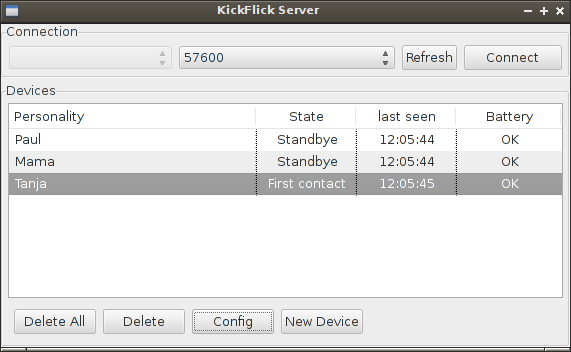
\includegraphics[width= 0.5\textwidth, clip=true  ,keepaspectratio=true]{./pic/java-server-main.png}
 % java-server-main.png: 0x0 pixel, 0dpi, nanxnan cm, bb=
 \caption{Main Window}
 \label{java-server-main}
\end{figure}

If the server detects an entity in the network, the user can select it in the device-table and open a configuration dialogue by either pressing the configuration button (located on the bottom of the table) or by clicking on the intended table's item. The configuration dialogue will then be opened where this particular device and its personality can be altered.
In practical use, the ''New Device'' button won't be clicked because each detected device by clicking on ''connect'' will create an own entry in the table with the default personality ''Paul''. But the ''New Device'' button has its authorization to be there for implementing or debugging operations.\newline
An other case are the ''Delete'' and ''Delete All'' buttons. They are really necessary to use in the daily employment. The ''Config''buttons functionality was already explained above. For an user, it is just quite easier to open a new dialogue via several ways.

\subsubsection{Configuration Dialogue}

The Configuration Dialogue provides all the information about the selected entity's state and allows the configuration of the entity's personality. 

The user can customize a personality or select one among the predefined personalities. But if the user creates a personality and then selects a predefined one, all the changes made so far will be overridden by the predefined personality. 

To cancel all changes, the user just has to click the cross in the very top - right corner. Then all personalities have their default (or last saved)settings.(see Figure ~\ref{fig:java-server-config01}). But if the user wants to save his changes, he just have to click on the ''save|close'' button in the down - right corner.    

In the Configuration Dialogue, the personality's settings are distributed in three different tabs. The tab ''Basic'' (see Figure ~\ref{fig:java-server-config01}) contains the personality's name, the addresses of the two nodes that constitute the entity and a table with all the possible action keys. Only the checked keys will be enabled in the entity; that is, the entity will only react to a certain action key if the latter has a check next to it in the table. Every key can be enabled and disabled by the user. 

By clicking on a device in the table of the main window, this first view of the configuration window opens. In the Default Configuration part of the window the chosen device will be shown with its device name. Because the user can overwrite the name of a personality, it was necessary to show the actuators and the sensors ID.
Furthermore the actual state of the device is prompted so that the user can change the behaviour of a device in a special state. 


\begin{figure}[h!]
 \centering
 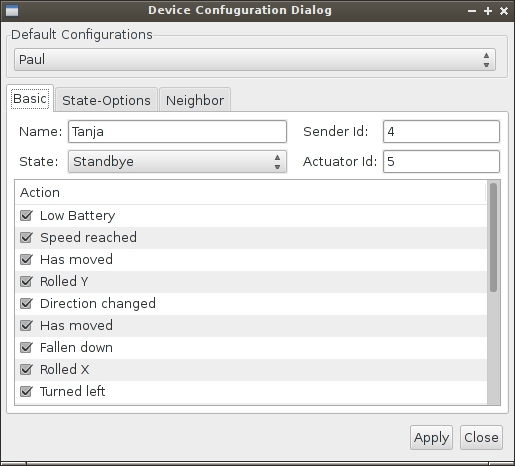
\includegraphics[width= 0.5\textwidth, clip=true  ,keepaspectratio=true]{./pic/java-server-config01.png}
 % java-server-main.png: 0x0 pixel, 0dpi, nanxnan cm, bb=
 \caption{Configuration Dialog, 1st Tab: Basic}
 \label{fig:java-server-config01}
\end{figure}

In the second tab of the Configuration Window the "Reaction Options" are set.
So the window is separated in an upper and a lower part. In the upper one the behaviour of the device can be set in the Standby (default) state. A personality's behaviour is interpolated by four objects: Once, there is a pattern (like blinking, fading, rainbow, ... ). This pattern needs two colours to switch between. At least, the behaviour needs a time (duration) for how long a pattern is.
In the lower part all other states can be manipulated.   


\begin{figure}[h!]
 \centering
 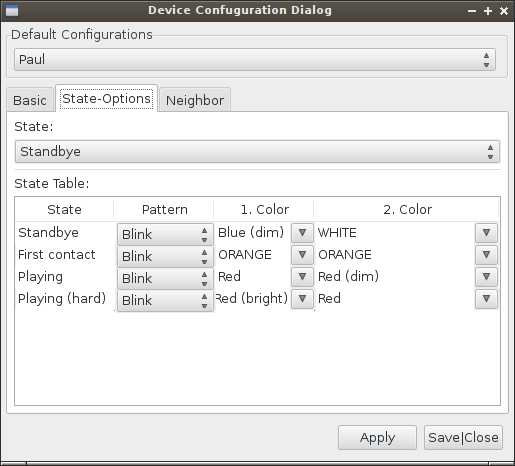
\includegraphics[width= 0.5\textwidth, clip=true  ,keepaspectratio=true]{./pic/java-server-config02.png}
 % java-server-main.png: 0x0 pixel, 0dpi, nanxnan cm, bb=
 \caption{Configuration Dialogue, 2nd Tab: Reaction Options}
 \label{fig:java-server-config02}
\end{figure}


Finally, the third tab labelled ''Neighbor'' displays the actions to be performed when the entity detects a neighbor (see Figure ~\ref{fig:java-server-config03}). The table shows the personality of each entity that has been detected by the server. However, if an entity has a preset personality, it will not be displayed in this tab since its reaction towards a neighbour is already defined and is not configurable. 

In this tab, the user can set the pattern and colors that the entity and its found neighbor will display. For instance, according to the settings in Figure ~\ref{fig:java-server-config03}, if the entity ''Paul'' is clicked in the users interface to its configuration window and the device finds another ''Paul'', both entities will exhibit a blink pattern with green and blue. Here, the duration time is constant.

In order to save the changes made to the personality's settings, the user has to press the ''save|close'' button like in the main window. Otherwise, if the dialogue is closed by pressing the x in the very right - top corner, no changes will be saved and the entities settings fall back to the last saved changes or the default. 

\begin{figure}[h!]
 \centering
 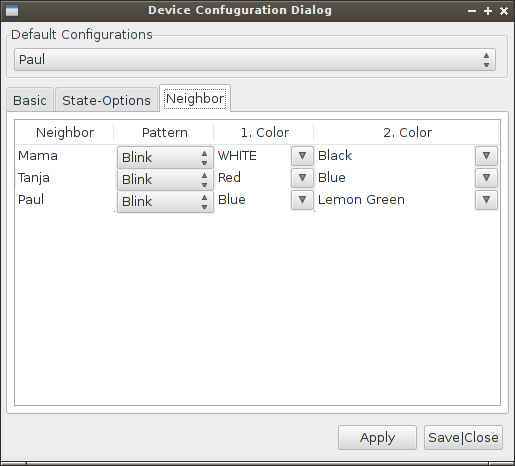
\includegraphics[width= 0.5\textwidth, clip=true  ,keepaspectratio=true]{./pic/java-server-config03.png}
 % java-server-main.png: 0x0 pixel, 0dpi, nanxnan cm, bb=
 \caption{Configuration Dialog, 3rd Tab: Neighbor}
 \label{fig:java-server-config03}
\end{figure}

\subsubsection{Interface Architecture}
The interface was created with the swt widget toolkit from eclipse. %insert cite
To periodically update the device table, the main window uses a swt timerevent. Every event-based action, like button clicks or selection were also implemented with the built-in event-listener structure of the swt toolkit. %insert cite again

When the dialogue is opened, the entity will be passed as a parameter in the constructor, the dialogue will then create the interface and afterwards read the entity's settings %Daniel, what do you mean by dialogue here? The Configuration Dialogue?

After changing one or more settings, if the user presses the ''apply'' button, these are kept in a temporal device. Then, if the ''save|close'' button is pressed, the new settings will be stored in a device instance that will be passed to the Main Window. When the user wants to discard the changes instead, he or she has to press the ''close'' button; the close action will pass a null pointer to the Main Window instance to indicate that no changes were committed. 

%The configuration will have no effect on the device at all, except the user says so. All changes will only be written when the apply button is pressed and even then a %temporally device will be created to first save all settings in the instance. If the user decides not to use the new settings and wants them to ignored, he then needs %to press the windows close button. The close action will pass a null pointer to the main window instance, signaling that no changes were commited.
%If, on the other hand, the user wants, after applying, to overwritte the device with the new settings he needs to close the configuration dialog by pressing the save %and close button. This will pass a device instance to the main window with all settings and therefor overwrite the previous settings of the device.

The Configuration Dialog widgets will be filled out on the creation of the dialog with all available data, e.g. reaction key names. After the interface is built, the device settings will be set. For example, this happens by setting the right selection for a combobox.
%I don't understand this paragraph :-(

The neighbor and state's tables are dynamically created; therefore, one can add more states and the number of possible neighbors is theoretically unlimited.


% vim: spell spelllang=en_gb 
